
%(BEGIN_QUESTION)
% Copyright 2010, Tony R. Kuphaldt, released under the Creative Commons Attribution License (v 1.0)
% This means you may do almost anything with this work of mine, so long as you give me proper credit

Dekod følgende serielle datastrømmer, der hver er kodet med en ulik metode:

$$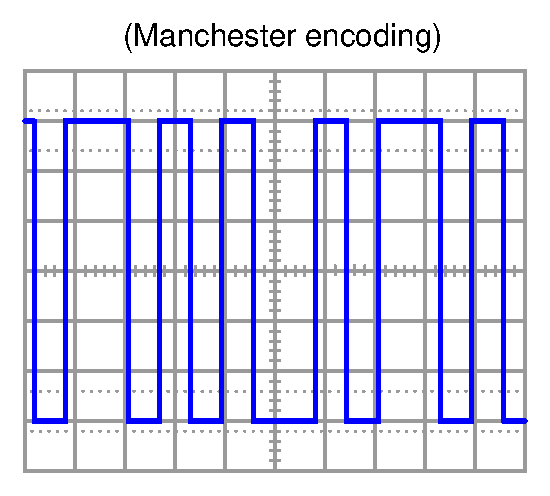
\includegraphics[width=15.5cm]{i00883x01.eps}$$

$$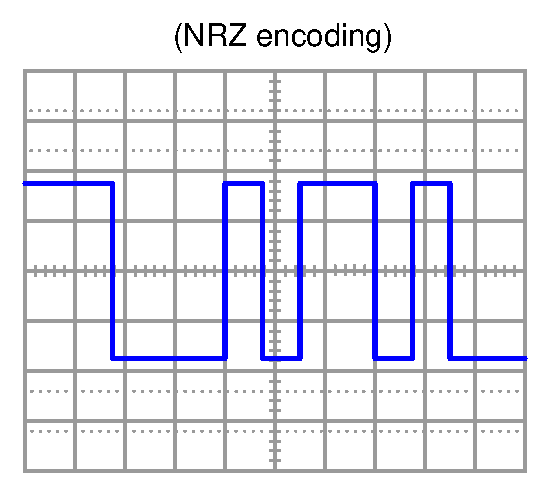
\includegraphics[width=15.5cm]{i00883x03.eps}$$

$$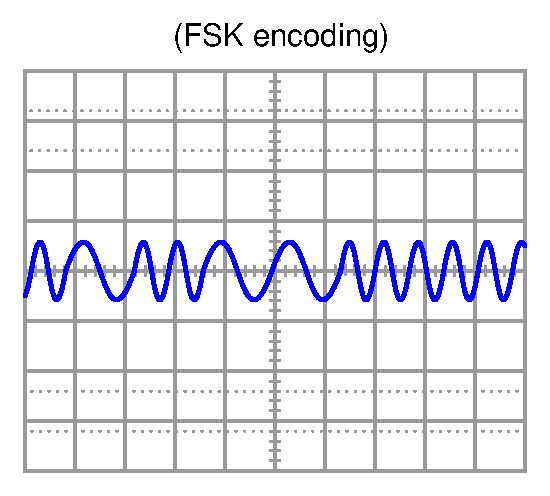
\includegraphics[width=15.5cm]{i00883x05.eps}$$

\vskip 20pt \vbox{\hrule \hbox{\strut \vrule{} {\bf Forslag til sokratisk diskusjon} \vrule} \hrule}

\begin{itemize}
\item{} Studenter opplever ofte forvirring ved tolkning av datastrømmer vist slik, spesielt Manchester-koding. En effektiv strategi er å {\it løse baklengs}: start med kjent datastrøm (1/0) og tegn bølgeformen den gir. Gjør dette for flere mønstre (repeterende bit vs. alternerende bit osv.), og se hvilke generelle regler som kan brukes for pålitelig tolkning.
\item{} Korrekt tolkning av NRZ krever korrekt måling av pulsbredden. Foreslå en metode når pulsene ikke ligger pent på oscilloskopets rutenett.
\item{} Forklar hvordan de tre kodemetodene tydelig viser forskjellen mellom {\it bit rate} og {\it baud}. Hvilken metode gir høyest bits/sekund per baud? Hvilken gir lavest?
\end{itemize}

\underbar{file i00883}
%(END_QUESTION)





%(BEGIN_ANSWER)

$$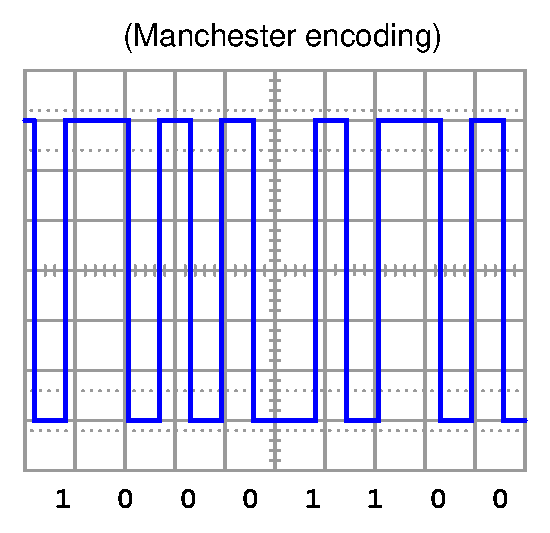
\includegraphics[width=15.5cm]{i00883x02.eps}$$

$$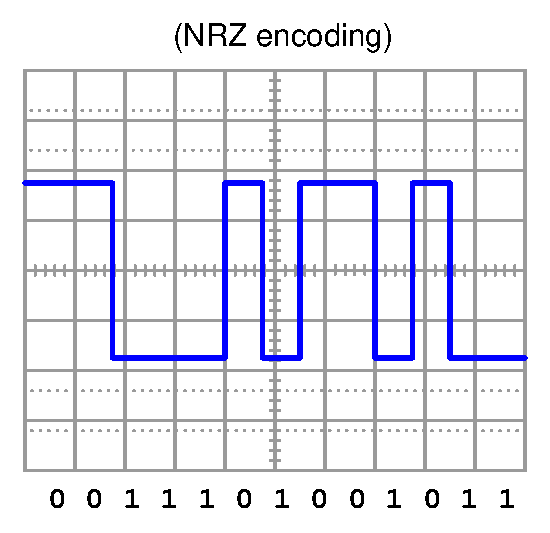
\includegraphics[width=15.5cm]{i00883x04.eps}$$

$$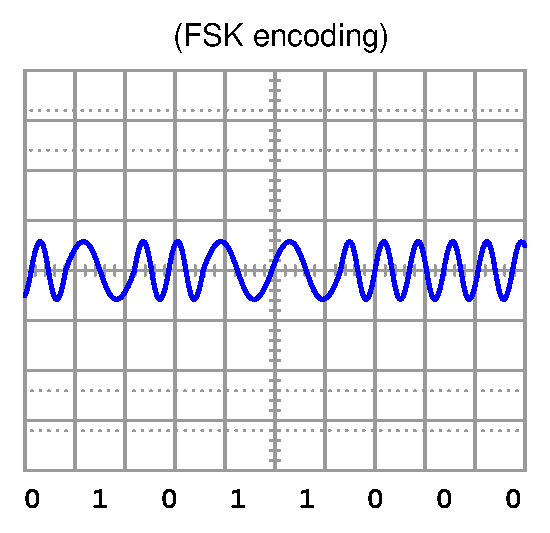
\includegraphics[width=15.5cm]{i00883x06.eps}$$

%(END_ANSWER)





%(BEGIN_NOTES)

Merk at bitrate for NRZ-kodet data i praksis kan være heltallsmultipler av det som vises. Med andre ord kan hver ``mark'' (1) og ``space'' (0) representere to, tre eller flere påfølgende bit. Vi har ingen sikker måte å vite dette uten en forhåndsdefinert bitrate.

%INDEX% Electronics review: NRZ encoding
%INDEX% Electronics review: Manchester encoding
%INDEX% Electronics review: FSK encoding

%(END_NOTES)
